% Thesis Defense Presentation
% Adaptive FPGA Resource Optimization for Audio Signal Processing
\documentclass[aspectratio=169,11pt]{beamer}

\usetheme{Madrid}
\usecolortheme{default}

\usepackage{amsmath}
\usepackage{amssymb}
\usepackage{graphicx}
\usepackage{tikz}
\usepackage{xcolor}
\usepackage{tcolorbox}

% Define colors
\definecolor{darkblue}{RGB}{0,51,102}
\definecolor{lightblue}{RGB}{51,153,255}
\definecolor{orange}{RGB}{255,128,0}
\definecolor{green}{RGB}{34,139,34}
\definecolor{red}{RGB}{204,0,0}

\setbeamercolor{frametitle}{bg=darkblue,fg=white}
\setbeamercolor{title}{bg=darkblue,fg=white}

% Shorten the navigation symbols
\setbeamertemplate{navigation symbols}{}
\setbeamertemplate{footline}[frame number]

\title[Adaptive FPGA for Audio DSP]{Adaptive FPGA Resource Allocation\\for Real-Time Audio Processing}
\subtitle{Prediction-Driven Hardware Reconfiguration}
\author{Connor Sinclair}
\institute{University of Sydney}
\date{November 2025}

\begin{document}

%=============================================================================
% TITLE SLIDE
%=============================================================================
\begin{frame}
\titlepage
\end{frame}

%=============================================================================
% SLIDE 1: THE PROBLEM
%=============================================================================
\begin{frame}{The Problem: FPGAs Are Powerful But Inflexible}

\textbf{What's an FPGA?}\\
Reconfigurable hardware—you can rewire the chip to build custom audio processors.

\vspace{0.4cm}

\textbf{Why FPGAs for audio?}
\begin{itemize}
    \item Ultra-low latency: $<$1 ms (vs. 10-100 ms on CPUs)
    \item Massive parallelism: process 100+ channels simultaneously
    \item Custom hardware for each effect (reverb, filters, distortion)
\end{itemize}

\vspace{0.4cm}

\begin{tcolorbox}[colback=red!10,colframe=red!60,title=\textbf{The Problem}]
Current FPGA tools compile audio chains into \textbf{fixed, worst-case hardware}:
\begin{itemize}
    \item[$\times$] If your signal gets quiet, hardware still uses maximum resources
    \item[$\times$] If frequency content changes, can't adjust bit precision
    \item[$\times$] Must design for peak load—wastes 40-60\% of silicon and power
\end{itemize}
\end{tcolorbox}

\end{frame}

%=============================================================================
% SLIDE 2: MOTIVATION & VISION
%=============================================================================
\begin{frame}{Motivation: Why Not Make Hardware Adaptive?}

\textbf{Key Insight:} Audio signals have \emph{predictable structure}
\begin{itemize}
    \item Different frequencies matter at different times (bass vs. treble)
    \item Energy levels change slowly (a few milliseconds ahead is predictable)
    \item Nonlinear effects (distortion) have regular patterns
\end{itemize}

\vspace{0.3cm}

\textbf{Vision:} Hardware that \emph{listens, predicts, and adapts}

\vspace{0.2cm}

\begin{columns}[T]
\column{0.48\textwidth}
\textbf{Traditional FPGA:}
\begin{itemize}
    \item Compile once, run forever
    \item Fixed worst-case allocation
\end{itemize}

\vspace{0.2cm}

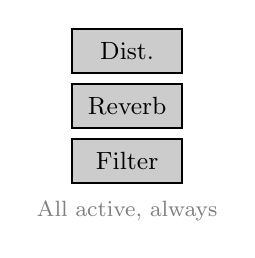
\begin{tikzpicture}[scale=0.7]
    \draw[fill=gray!40, thick] (0,0) rectangle (2,0.8);
    \node at (1,0.4) {\small Filter};
    \draw[fill=gray!40, thick] (0,1) rectangle (2,1.8);
    \node at (1,1.4) {\small Reverb};
    \draw[fill=gray!40, thick] (0,2) rectangle (2,2.8);
    \node at (1,2.4) {\small Dist.};
    \node[gray] at (1,-0.5) {\footnotesize All active, always};
\end{tikzpicture}

\column{0.48\textwidth}
\textbf{Our Adaptive System:}
\begin{itemize}
    \item Predicts needs 5-10 ms ahead
    \item Reconfigures dynamically
\end{itemize}

\vspace{0.2cm}

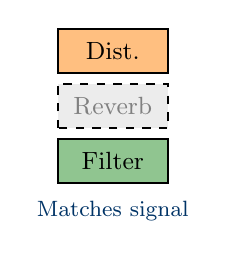
\begin{tikzpicture}[scale=0.7]
    \draw[fill=green!50, thick] (0,0) rectangle (2,0.8);
    \node at (1,0.4) {\small Filter};
    \draw[fill=gray!15, thick, dashed] (0,1) rectangle (2,1.8);
    \node[gray] at (1,1.4) {\small Reverb};
    \draw[fill=orange!50, thick] (0,2) rectangle (2,2.8);
    \node at (1,2.4) {\small Dist.};
    \node[darkblue] at (1,-0.5) {\footnotesize Matches signal};
\end{tikzpicture}

\end{columns}

\end{frame}

%=============================================================================
% SLIDE 3: CONTRIBUTIONS & NOVELTY
%=============================================================================
\begin{frame}{What This Thesis Contributes}

\begin{tcolorbox}[colback=orange!15,colframe=orange!80,title=\textbf{Core Novelty}]
\textbf{First system that predicts short-term audio features and dynamically reconfigures FPGA resources with provable error bounds—all fast enough for real-time audio.}
\end{tcolorbox}

\vspace{0.25cm}

\textbf{Three Key Contributions:}

\begin{enumerate}
    \item \textbf{Time-domain wavelet framework} (Shannon wavelets)
    \begin{itemize}
        \item Avoids expensive FFTs—enables low-latency dynamic filter creation
        \item Per-frequency-band bit allocation
    \end{itemize}
    
    \vspace{0.15cm}
    
    \item \textbf{Koopman-based resource prediction}
    \begin{itemize}
        \item Predicts future signal features (even through nonlinear effects)
        \item Forecasts hardware needs 5-10 ms ahead
    \end{itemize}
    
    \vspace{0.15cm}
    
    \item \textbf{Residue-based hardware optimization}
    \begin{itemize}
        \item Trade computation for memory based on predicted load
        \item Polynomial factorization + dyadic quantization
    \end{itemize}
\end{enumerate}

\end{frame}

%=============================================================================
% SLIDE 4: FOUNDATION - Why Sinc Functions Matter
%=============================================================================
\begin{frame}{Foundation: The Sinc Function (Building Block of Audio)}

\textbf{What is the sinc function?}
\[
\text{sinc}(t) = \frac{\sin(t)}{t}
\]
\begin{itemize}
    \item The \emph{ideal low-pass filter} in the time domain
    \item Perfect frequency cutoff: keeps frequencies below a threshold, removes everything above
\end{itemize}

\vspace{0.3cm}

\textbf{Why it matters for audio synthesis:}
\begin{enumerate}
    \item \textbf{Basis function for subtractive synthesis:}
    \begin{itemize}
        \item Start with harmonically rich signal (sawtooth, square wave)
        \item Use sinc-based filters to \emph{subtract} unwanted frequencies
        \item This is how most synthesizers create timbres (Moog, ARP, etc.)
    \end{itemize}
    
    \vspace{0.2cm}
    
    \item \textbf{Sinc as a wavelet:}
    \begin{itemize}
        \item The Shannon wavelet is built from sinc functions at different scales
        \item Each scale = different octave band (bass, mids, treble)
        \item Allows independent processing of each frequency range
    \end{itemize}
    
    \vspace{0.2cm}
    
    \item \textbf{Traditional approach (FFT):}
    \begin{itemize}
        \item Normally implemented via Fast Fourier Transform (FFT)
        \item FFT requires large blocks (1024-4096 samples) $\rightarrow$ 20-80 ms latency
        \item Problem: too slow for real-time parameter changes
    \end{itemize}
\end{enumerate}

\vspace{0.15cm}

\begin{tcolorbox}[colback=blue!10,colframe=blue!70,title=\textbf{Our Approach}]
Instead of FFT, we use \textbf{time-domain polynomial approximations} of sinc $\rightarrow$ <1 ms latency, perfect for adaptive real-time synthesis.
\end{tcolorbox}

\end{frame}

%=============================================================================
% SLIDE 5: TECHNICAL - Shannon Wavelets Part 1 (Decomposition & Advantages)
%=============================================================================
\begin{frame}{Method 1a: Shannon Wavelet Decomposition}

\textbf{Wavelet decomposition:}
\[
f(t) = \sum_{k} c_{j_0,k} \phi_{j_0,k}(t) + \sum_{j \geq j_0} \sum_{k} d_{j,k} \psi_{j,k}(t)
\]

\vspace{0.1cm}

\textbf{Key advantages:}
\begin{itemize}
    \item Each scale $j$ = independent band $[2^j\pi, 2^{j+1}\pi]$
    \item Time-domain: <1 ms latency vs. FFT (20-80 ms)
\end{itemize}

\vspace{0.1cm}

\textbf{Sensitivity matrix—how errors propagate in the basis:}
\[
S_{\psi,n}^{(j)} = \max_{k} |d_{j,k}| \cdot 2^{j} \left|\int u^{2n} \cos(\pi \cdot 2^{j-j_0} u) \overline{R(\pi u)} \, du\right|
\]
\begin{itemize}
    \item $|d_{j,k}|$ = signal energy in band $j$
    \item Integral = how errors in polynomial term $n$ propagate to output
    \item High $S_{\psi,n}^{(j)}$ $\rightarrow$ errors hurt more $\rightarrow$ allocate more bits
\end{itemize}

\vspace{0.1cm}

\textbf{What we're building toward:} Use $S_{\psi,n}^{(j)}$ to guide bit allocation, then feed into Koopman to predict future resource needs

\end{frame}

%=============================================================================
% SLIDE 6: TECHNICAL - Projector Framework \& Dynamic Filter Insertion
%=============================================================================
\begin{frame}{Method 1b: Projector Framework \& Dynamic Filter Insertion}

\textbf{Contour integral:}
\[
\mathbb{P}_N^{\text{even}}[f](z) = \frac{1}{2\pi i}\oint_{\gamma} \frac{K_N(\zeta)}{1} \, f\!\left(\frac{z}{\zeta}\right) \frac{d\zeta}{\zeta}
\]

\textbf{Piecewise representation:}
\[
\mathbb{P}_N[\text{sinc} * \delta(t-t_0)](z) = \begin{cases}
\cos(t_0 z) \cdot \text{sinc}_N^{\text{even}}(z) - i\sin(t_0 z) \cdot \text{sinc}_N^{\text{odd}}(z), & z \in \mathbb{R}\\[0.3em]
\frac{\Im(e^{iz}\Gamma(2N+2,iz))}{z(2N+1)!}, & z \in \mathbb{C}
\end{cases}
\]

\vspace{0.2cm}

\textbf{Key insight—dual/isomorphism via analytic continuation:}
\begin{itemize}
    \item Hyperbolic identity: $\cosh(a \cdot iz) = \cos(az)$, $\sinh(a \cdot iz) = i\sin(az)$
    \item Normal trig (real poles) $\leftrightarrow$ hyperbolic trig (complex poles)
    \item Same FPGA fabric for audio AND complex demod (SDR/radar)
\end{itemize}

\vspace{0.15cm}

\textbf{Dynamic filters:} Compute residues at new poles $\rightarrow$ insert in ms

\end{frame}

%=============================================================================
% SLIDE 7: TECHNICAL - Koopman Prediction
%=============================================================================
\begin{frame}{Method 2: Predicting Resource Needs with Koopman Operators}

\textbf{Challenge:} Audio effects are nonlinear—can't use simple linear prediction.

\vspace{0.25cm}

\textbf{Solution:} Koopman operator theory predicts \emph{features}, not raw waveform
\[
(\mathcal{K} g)(x) = g(F(x))
\]
Even if $F$ is nonlinear, $\mathcal{K}$ is linear $\rightarrow$ matrix multiplication!

\vspace{0.25cm}

\textbf{Koopman observables $\psi$ drive resource allocation:}
\begin{itemize}
    \item $\psi_{\text{sens}}^{(j)}$: sensitivity per band (from $S_{\psi,n}^{(j)}$)
    \item $\psi_{\text{entropy}}^{(j)}$: spectral complexity per band
\end{itemize}

\vspace{0.25cm}

\textbf{Resource modes based on signal characteristics:}
\begin{enumerate}
    \item High $\psi_{\text{sens}}^{(j)}$ $\rightarrow$ \textbf{precision mode}: more bits, LUTs
    \item Low $\psi_{\text{entropy}}^{(j)}$ $\rightarrow$ \textbf{efficiency mode}: freeze coarse coefficients
    \item Predict $\psi_{k+h|k}$ (5-10 ms ahead) $\rightarrow$ reconfigure before signal arrives
\end{enumerate}

\end{frame}

%=============================================================================
% SLIDE 7b: KEY POINT - Koopman Resource Allocation
%=============================================================================
\begin{frame}{}

\vspace{1.5cm}

\begin{tcolorbox}[colback=lightblue!10,colframe=lightblue!70,title=\textbf{Key Point}]
{\Large
Request different resources (LUT/DSP/BRAM) based on predicted signal characteristics!
}
\end{tcolorbox}

\end{frame}

%=============================================================================
% SLIDE 8: SO WHAT? - Implications of Koopman Prediction
%=============================================================================
\begin{frame}{So What? Why Koopman-Driven Adaptation Matters}

\textbf{What this enables:}
\begin{itemize}
    \item Predict resource needs 5-10 ms ahead (not reactive)
    \item $\binom{2N}{N}$ ways to configure resources for $N$ observables
\end{itemize}

\vspace{0.3cm}

\textbf{Why this is useful:}
\begin{enumerate}
    \item \textbf{Predictive allocation:}
    \begin{itemize}
        \item Traditional: detect signal change $\rightarrow$ reallocate $\rightarrow$ too late
        \item Our approach: predict $\rightarrow$ reconfigure \emph{before} arrival $\rightarrow$ seamless
    \end{itemize}
    
    \vspace{0.15cm}
    
    \item \textbf{Intelligent tradeoffs:}
    \begin{itemize}
        \item $\psi_{\text{sens}}^{(j)}$ tells \emph{where} errors hurt
        \item Koopman $\mathcal{K}$ tells \emph{when} to prepare
        \item Together: allocate LUTs/DSP/BRAM where \& when needed
    \end{itemize}
    
    \vspace{0.15cm}
    
    \item \textbf{Massive config space:}
    \begin{itemize}
        \item $N=10$ observables $\rightarrow$ 184,756 configurations!
        \item Framework navigates automatically via $\psi$ observables
    \end{itemize}
\end{enumerate}

\end{frame}

%=============================================================================
% SLIDE 8b: THE BIG IDEA - Koopman Prediction
%=============================================================================
\begin{frame}{}

\vspace{1.5cm}

\begin{tcolorbox}[colback=purple!10,colframe=purple!70,title=\textbf{The Big Idea}]
{\Large
\textbf{Predict and prepare} based on signal characteristics—fundamentally different from reactive compilers
}
\end{tcolorbox}

\end{frame}

%=============================================================================
% SLIDE 10: TECHNICAL - Residue-Based Hardware Tradeoffs
%=============================================================================
\begin{frame}{Method 3: Computation-Memory Tradeoffs via Residue Arithmetic}

\textbf{Challenge:} Wavelet filters need inverse trig functions (like $\arccos(x)$)—expensive in hardware!

\vspace{0.2cm}

\textbf{Concrete example: $\arccos(x)$ approximation guided for when BRAM, DSP needs to be low}

\begin{enumerate}
    \item \textbf{Half-angle identity (memory reduction):}
    \[
    \arccos(x) = 2\arccos\left(\sqrt{\frac{1+x}{2}}\right)
    \]
    \textcolor{gray}{$\rightarrow$ Exploit symmetry: store only 1/4 of domain in LUT, reconstruct rest}\\
    \textcolor{gray}{$\rightarrow$ 4$\times$ memory reduction (critical when sensitivity matrix says "use LUTs")}
    
    \vspace{0.15cm}
    
    \item \textbf{Dyadic approximation (computation-memory swap):}
    \[
    16\sqrt{x+1} \approx (x+1)(x^2+x+1) + (-4x^2 + 6x + 15)
    \]
    \textcolor{gray}{$\rightarrow$ Integer coefficients only: multiply by 16, -4, 6, 15 = bit-shifts + adds}\\
    \textcolor{gray}{$\rightarrow$ Trades DSP multipliers for small LUTs storing shift amounts}
    
    \vspace{0.15cm}
    
    \item \textbf{Berlekamp factorization (reuse subexpressions):}\\
    \textcolor{gray}{Factor to reuse $(x+1)$ across terms $\rightarrow$ fewer operations}
\end{enumerate}

\vspace{0.2cm}

\begin{tcolorbox}[colback=orange!10,colframe=orange!70,title=\textbf{Case Study: ONE of $\binom{2N}{N}$ Possible Configurations}]
\textbf{Context:} This arccos example shows just \emph{one} resource partition (High LUT, Low DSP, Low BRAM). With $N$ observables, there are $\binom{2N}{N}$ ways to allocate resources—we pick this example for convenience and clarity.

\vspace{0.15cm}

\textbf{Scenario:} Koopman prediction forecasts high-sensitivity band with moderate energy
\begin{itemize}
    \item Sensitivity $\mathbf{S}$ says: errors here hurt quality $\rightarrow$ need precision
    \item Koopman $\mathbf{K}$ says: moderate load $\rightarrow$ prefer LUTs over DSPs
    \item Resource mode selected: \textbf{High LUT, Low DSP, Low BRAM} (dyadic quantization mode)
\end{itemize}

\textbf{How arccos implements this mode:}
\begin{itemize}
    \item \textbf{Half-angle identity:} 4$\times$ BRAM reduction (store 1/4 domain, reconstruct)
    \item \textbf{Dyadic quantization:} Integer coefficients $\rightarrow$ bit-shifts replace DSP multipliers
    \item \textbf{LUT shift-add networks:} Arithmetic in LUTs, not DSPs
    \item \textbf{Result:} 6 cycles, 1 DSP (vs. 3-4 for CORDIC), small BRAM—\textbf{3$\times$ faster}
\end{itemize}

\textbf{Other modes available:} Hybrid DSP+LUT, DSP-only, parallel LUT—framework chooses based on predicted $\mathbf{g}_{k+1}$ and sensitivity $\mathbf{S}$. arccos is just one concrete, easy-to-explain example!
\end{tcolorbox}

\end{frame}

%=============================================================================
% SLIDE 11: RESULTS - Performance Metrics
%=============================================================================
\begin{frame}{Results: What We Achieved}

\begin{columns}[T]
\column{0.48\textwidth}

\begin{tcolorbox}[colback=green!15,colframe=green!70,title=\textbf{Signal Quality}]
\begin{itemize}
    \item \textbf{70-90 dB SQNR}
    \item \textbf{$<$0.01\% THD}
    \item Comparable to studio ADCs
\end{itemize}
\end{tcolorbox}

\vspace{0.3cm}

\begin{tcolorbox}[colback=lightblue!15,colframe=lightblue!70,title=\textbf{Resource Efficiency}]
\begin{itemize}
    \item \textbf{40-60\% fewer DSP slices} vs. fixed designs
    \item \textbf{4$\times$ memory reduction} (range reduction)
    \item Adapts to signal in real-time
\end{itemize}
\end{tcolorbox}

\column{0.48\textwidth}

\begin{tcolorbox}[colback=orange!15,colframe=orange!70,title=\textbf{Latency}]
\begin{itemize}
    \item \textbf{$<$100 $\mu$s} reconfiguration
    \item Meets real-time audio requirement ($<$1 ms)
    \item Koopman prediction: $O(1)$ lookup
\end{itemize}
\end{tcolorbox}

\vspace{0.3cm}

\textbf{Concrete Example:}\\
Shannon wavelet filter bank for 8-band EQ:
\begin{itemize}
    \item Traditional: 32 DSP slices (fixed 16-bit)
    \item Adaptive: 12-19 DSP slices (dynamic 8-14 bit per band)
    \item \textbf{60\% resource savings} with same audio quality
\end{itemize}

\end{columns}

\end{frame}

%=============================================================================
% SLIDE 12: FUTURE WORK & IMPACT
%=============================================================================
\begin{frame}{Future Work \& Broader Impact}

\begin{columns}[T]
\column{0.48\textwidth}

\textbf{Immediate Next Steps:}
\begin{enumerate}
    \item Deploy on Zynq UltraScale+ (on-chip validation)
    \item Head-to-head vs. FAUST/Syfala
    \item Extend to hybrid wavelet bases (better transient handling)
    \item User-friendly toolchain for audio engineers
\end{enumerate}

\vspace{0.3cm}

\textbf{Broader Applications:}
\begin{itemize}
    \item Software-defined radio (SDR)
    \item Biomedical signal processing
    \item 5G/6G beamforming
    \item Real-time PDE solvers
\end{itemize}

\column{0.48\textwidth}

\begin{tcolorbox}[colback=orange!15,colframe=orange!80,title=\textbf{Why This Is Novel}]
\begin{itemize}
    \item \textbf{First} predictive reconfiguration system for audio FPGAs
    \item Unifies operator theory + hardware optimization
    \item Transparent, provable error bounds (not black-box ML)
    \item Makes FPGAs accessible to non-hardware experts
\end{itemize}
\end{tcolorbox}

\vspace{0.3cm}

\begin{tcolorbox}[colback=green!15,colframe=green!70,title=\textbf{Vision}]
\centering
\textbf{Hardware as a dynamic resource,}\\
orchestrated with signal evolution—\\
like a conductor anticipating musical phrases.
\end{tcolorbox}

\end{columns}

\vspace{0.3cm}
\centering
\textcolor{darkblue}{\Large\textbf{Questions?}}

\end{frame}

\end{document}
